\section{Ergebnisse}
\label{sec:ergebnisse}

Die zentralen Forschungsfragen dieser Arbeit adressieren die Effektivität von Cross-Attention-Modellen im Vergleich zu etablierten Baselines, den Einfluss der Positionierung des Fusionsblocks sowie die Generalisierbarkeit der Ansätze. Dieser Abschnitt präsentiert die quantitativen und qualitativen Ergebnisse der durchgeführten Experimente. Zunächst werden die Resultate des Hauptexperiments analysiert, gefolgt von einer detaillierten Betrachtung der Ablationsstudien. Abschließend wird eine exemplarische Explainability-Analyse durchgeführt, um die Interaktion zwischen Text- und Tabulardaten zu illustrieren.

\subsection{Hauptexperiment}
\label{sec:hauptexperiment}

Im Hauptexperiment (Seed 777) wurde die Klassifikationsleistung der verschiedenen Architekturen auf dem primären Datensatz evaluiert. Tabelle \ref{tab:main_results} fasst die zentralen Metriken zusammen. Neben der Klassifikationsleistung (AUC und Average Precision) wird auch die Modellkomplexität (FLOPs und Parameteranzahl) verglichen.

\begin{table}[ht]
    \centering
    \small
    \caption{Vergleich der Hauptmetriken auf dem Testdatensatz (Seed 777). Hervorgehobene Werte markieren das beste Ergebnis pro Metrik.}
    \label{tab:main_results}
    \begin{tabular}{lcccc}
        \hline
        \textbf{Modell} & \textbf{AUC} & \textbf{AP} & \textbf{FLOPs} & \textbf{Parameter} \\
         & \textbf{(Test)} & \textbf{(Test)} & & \\
        \hline
        ConcatBERT & 0{,}9580 & 0{,}579 & $3{,}407 \cdot 10^{12}$ & 110 M \\
        SumBERT & 0{,}9727 & 0{,}601 & $3{,}407 \cdot 10^{12}$ & 110 M \\
        CrossBERT Early & 0{,}9743 & \textbf{0{,}620} & $3{,}408 \cdot 10^{12}$ & 118 M \\
        CrossBERT Late & 0{,}9746 & 0{,}614 & $3{,}408 \cdot 10^{12}$ & 118 M \\
        CrossBERT Hybrid & 0{,}9737 & 0{,}619 & $3{,}409 \cdot 10^{12}$ & 123 M \\
        \hline
    \end{tabular}
\end{table}

Zur Validierung der Robustheit wurden die Experimente mit einem alternativen Random Seed (333) wiederholt. Die Ergebnisse bestätigen die grundlegenden Trends des Hauptexperiments (siehe Anhang \ref{app:seed_333_evaluation}).

Abbildung \ref{fig:metrics_plots_baseline} und Abbildung \ref{fig:metrics_plots_cross_bert} zeigen die Verläufe der Trainings- und Validierungsmetriken für die Baseline-Modelle sowie die CrossBERT-Varianten.

\begin{figure}[h]
    \centering
    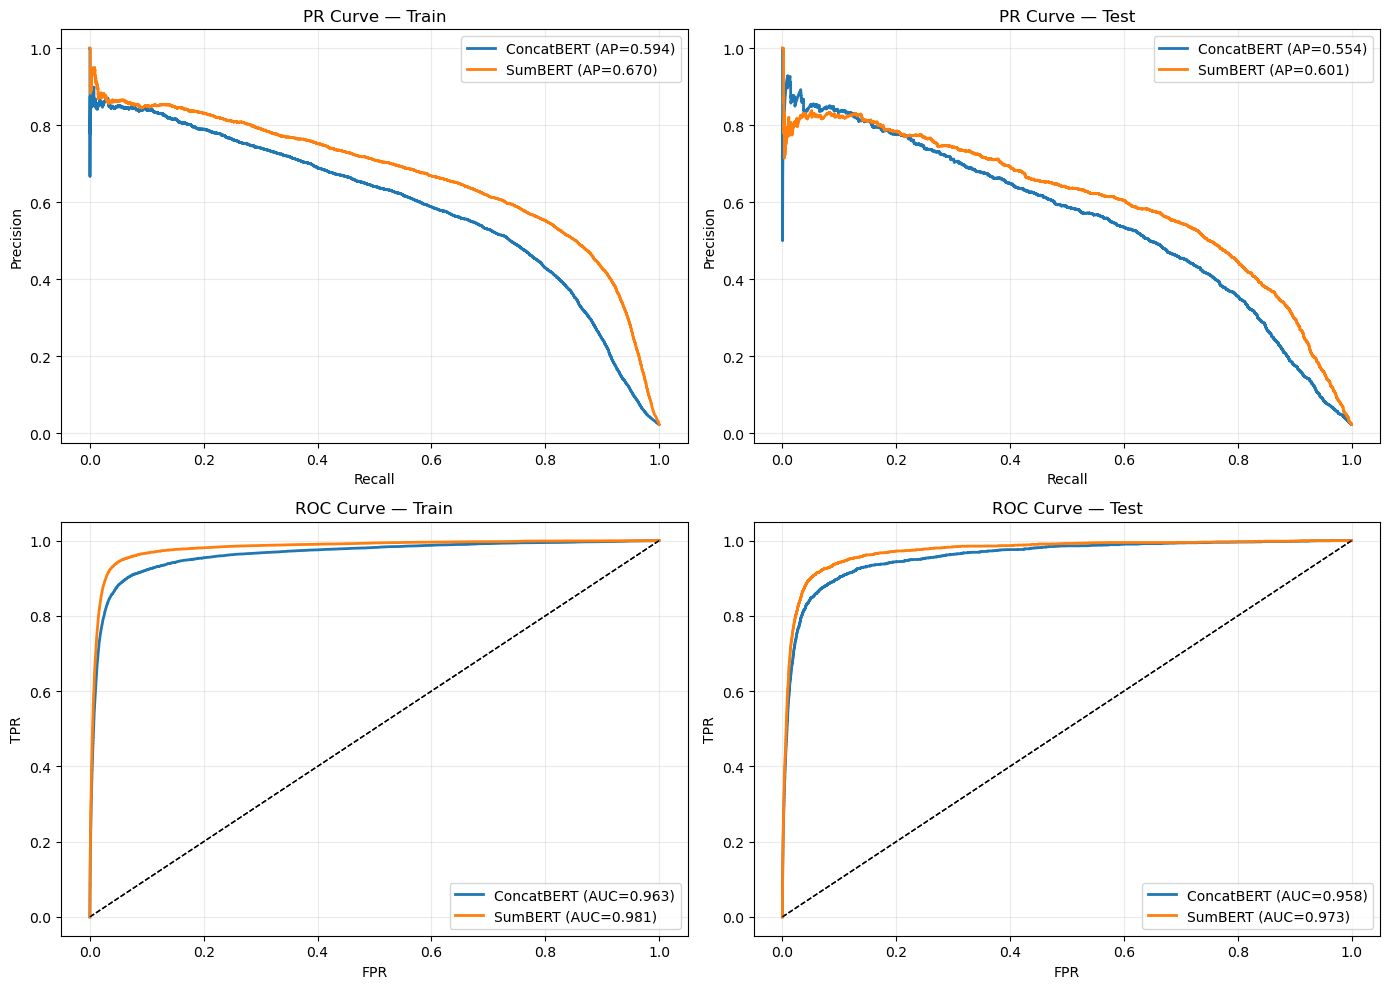
\includegraphics[width=\textwidth]{Bilder/metrics_plots_baseline.png}
    \caption{Trainingsverlauf der Baseline-Modelle (ConcatBERT und SumBERT).}
    \label{fig:metrics_plots_baseline}
\end{figure}

\begin{figure}[h]
    \centering
    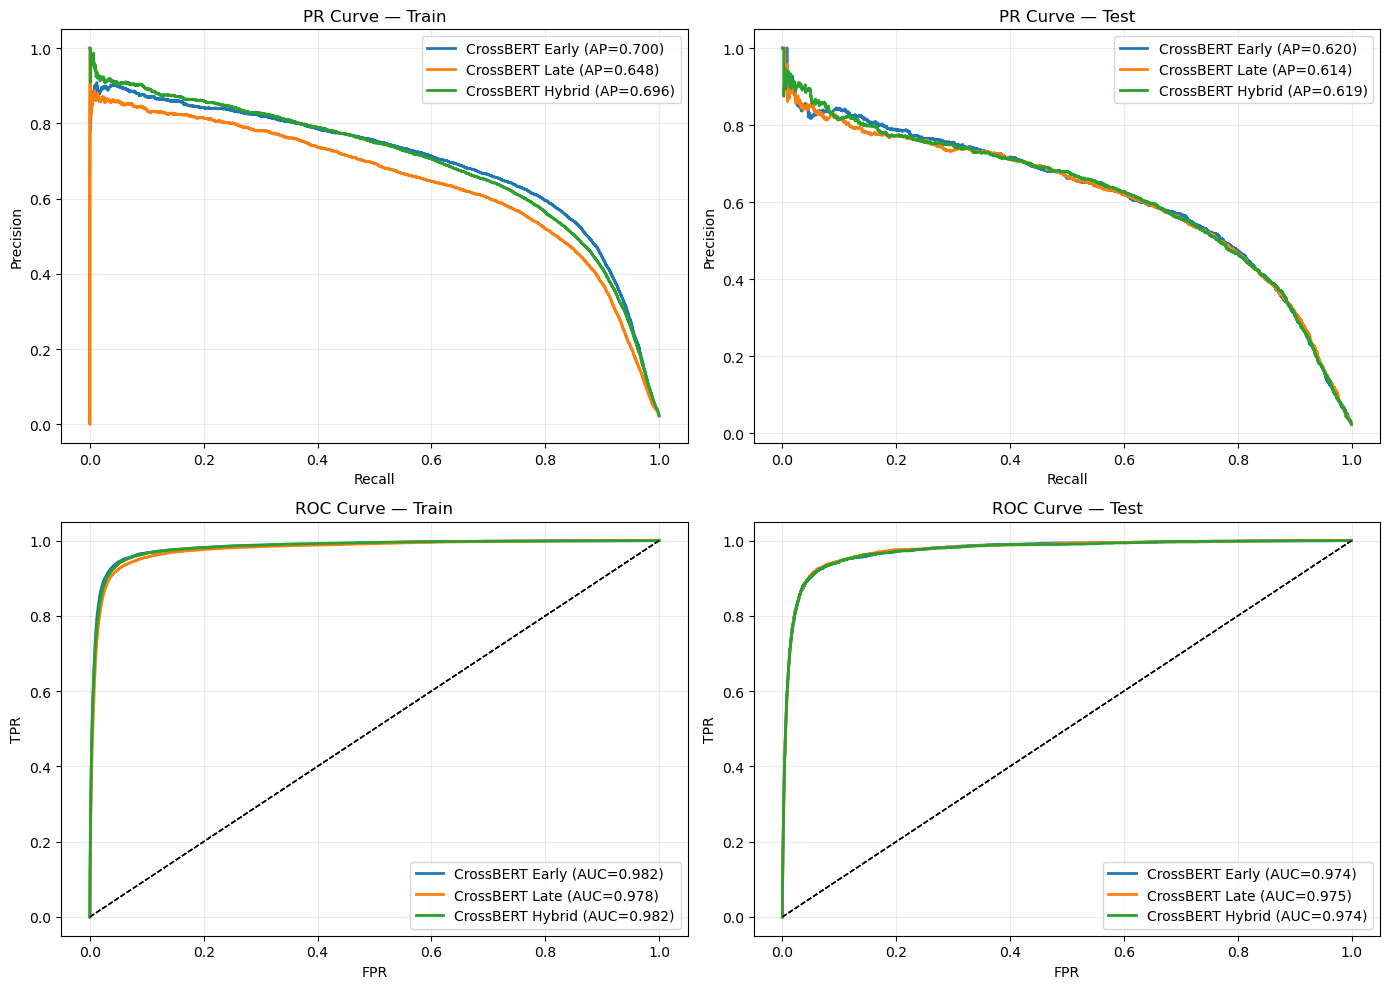
\includegraphics[width=\textwidth]{Bilder/metrics_plots_cross_bert.png}
    \caption{Trainingsverlauf der CrossBERT-Modelle.}
    \label{fig:metrics_plots_cross_bert}
\end{figure}

\subsection{Ablationsstudien}
\label{sec:ergebnisse_ablations}

Um den Einfluss spezifischer Designentscheidungen zu isolieren, wurden gezielte Ablationsstudien durchgeführt. Im Fokus stehen die Positionierung der Cross-Attention, die Anzahl der Tabular Tokens sowie methodische Erweiterungen wie der TabTokenizer V2 und Gating-Mechanismen.

\subsubsection{Einfluss der Cross-Attention-Positionierung}
\label{sec:res_ablation_position}

Die Positionierung des Cross-Attention-Blocks (Early, Late, Hybrid) zeigt einen signifikanten Einfluss auf die Modellleistung, insbesondere auf die Average Precision (vgl. Tabelle \ref{tab:main_results}).

\begin{figure}[h]
    \centering
    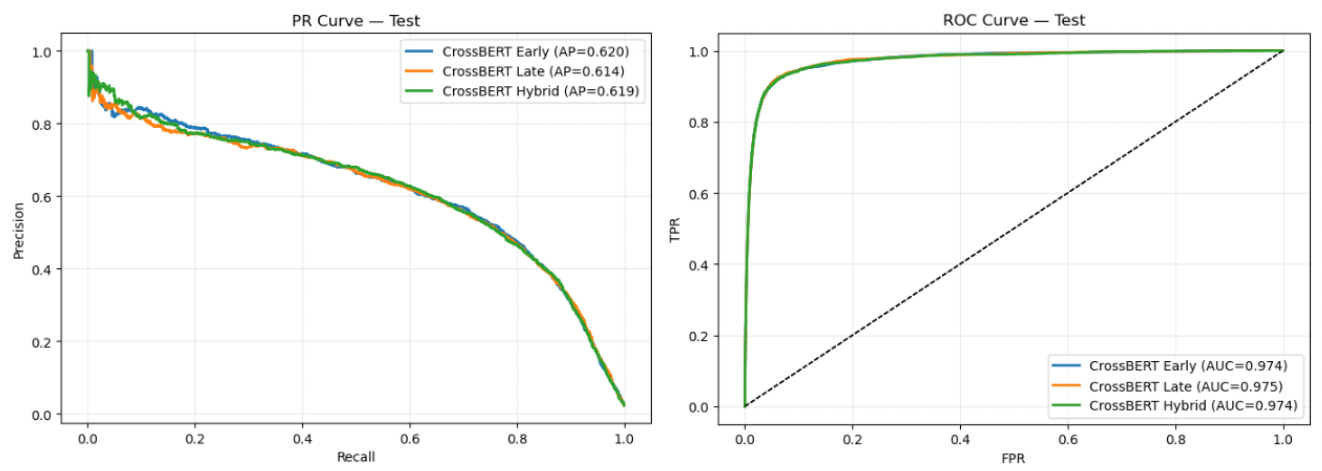
\includegraphics[width=\textwidth]{Bilder/CrossBERT_plots_positions.png}
    \caption{Vergleich der Metrik-Verläufe für CrossBERT Early, Late und Hybrid.}
    \label{fig:crossbert_plots_positions}
\end{figure}

\subsubsection{Einfluss der Anzahl der Tabular Tokens}
\label{sec:res_ablation_tokens}

Wie in Anhang \ref{app:ablation_num_tokens} detailliert dargestellt, wurde die Sensitivität des Modells gegenüber der Anzahl der Tabular Tokens ($n_{tab}$) untersucht. Die Ergebnisse zeigen, dass eine Erhöhung der Token-Anzahl bis zu einem gewissen Punkt ($n_{tab}=8$) die Performance stabilisiert, während extrem hohe oder niedrige Werte zu Einbußen führen können. Dies deutet darauf hin, dass die Positionierung der Cross-Attention allein nicht ausreicht – auch die Repräsentation der tabularen Daten interagiert maßgeblich mit der Fusionsarchitektur.

\subsubsection{Tabular Tokenizer V2 und Gating}
\label{sec:res_ablation_extensions}

Die Untersuchung des Tabular Tokenizers V2 (siehe Anhang \ref{app:ablation_tokenizer_v2}) und des Gating-Mechanismus (siehe Anhang \ref{app:ablation_gating}) zeigt, dass diese Erweiterungen in bestimmten Konfigurationen (z.B. Late Fusion) Vorteile bieten können, im Hybrid-Setup jedoch keine signifikante Verbesserung gegenüber der Basis-Variante erzielen.

\subsection{Externe Validierung}
\label{sec:res_external_validation}

Zur Überprüfung der Generalisierungsfähigkeit wurden die Modelle auf zwei weiteren Datensätzen evaluiert: dem Petfinder-Datensatz (ordinales Regressionsproblem) und einem E-Commerce-Datensatz (Sentiment-Analyse). Die detaillierten Ergebnisse finden sich in Anhang \ref{app:petfinder_evaluation} und Anhang \ref{app:ecommerce_evaluation}. Zusammenfassend bestätigt die externe Validierung, dass die CrossBERT-Architekturen, insbesondere die Hybrid-Variante, auch auf neuen Domänen robust performen.

\subsection{Illustrative Explainability-Analyse}
\label{sec:res_explainability}

Die folgende Analyse dient der exemplarischen Illustration, wie Cross-Attention und strukturierte Merkmale in einzelnen Vorhersagen interagieren. Sie erhebt keinen Anspruch auf statistische Repräsentativität, sondern soll die Modellmechanik veranschaulichen. Obwohl CrossBERT Early die höchste Average Precision erzielte, wird für diese Analyse das Hybrid-Modell herangezogen, da es über alle Metriken hinweg eine konsistente Leistung zeigte.

\subsubsection{Good Case: Korrekte Klassifikation mit hoher Konfidenz}
Im korrekt klassifizierten Fall mit hoher Konfidenz zeigen die SHAP-Werte eine konsistente Dominanz mehrerer strukturierter Merkmale. Die Cross-Attention verteilt sich vergleichsweise gleichmäßig über die tabularen Token, was auf eine integrierte Nutzung beider Modalitäten hindeutet.

\begin{figure}[h]
    \centering
    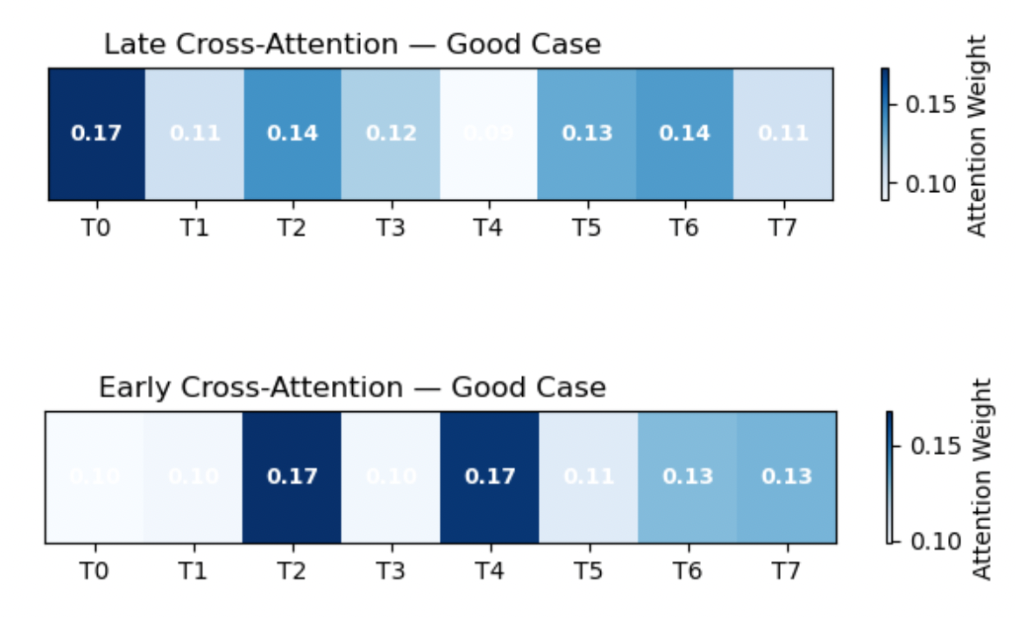
\includegraphics[width=0.8\textwidth]{Bilder/attention_good_case.png}
    \caption{Attention-Weights im Good Case.}
    \label{fig:attention_good_case}
\end{figure}

\begin{figure}[h]
    \centering
    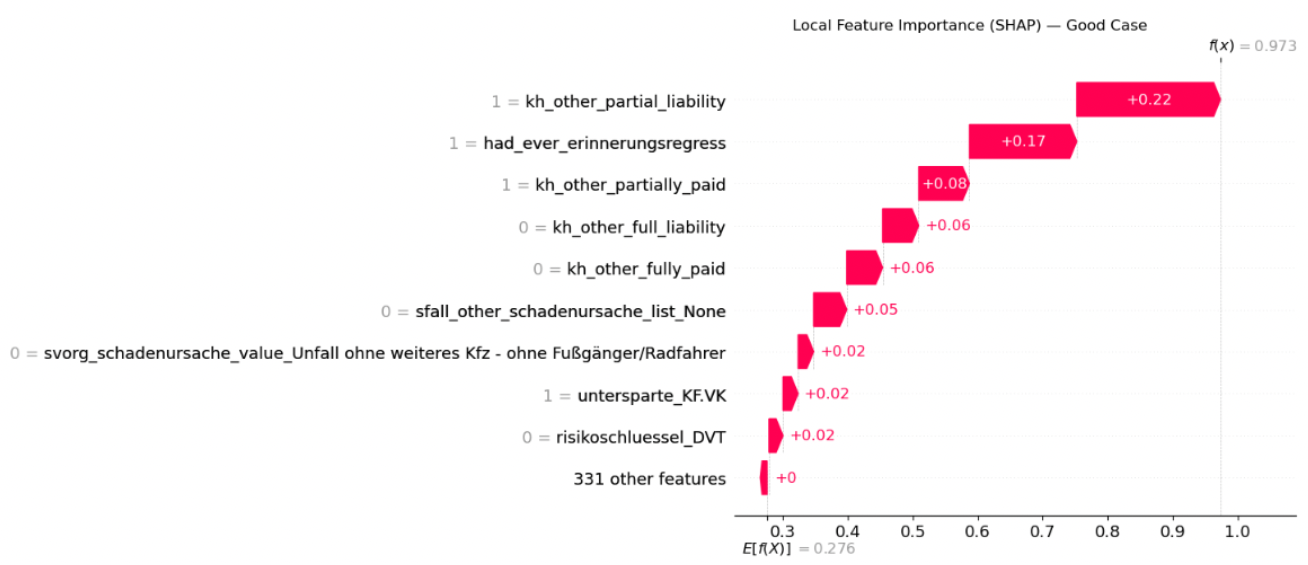
\includegraphics[width=0.8\textwidth]{Bilder/feature_importance_good_case.png}
    \caption{Feature Importance (SHAP) im Good Case.}
    \label{fig:feature_importance_good_case}
\end{figure}

\subsubsection{Bad Case: Fehlklassifikation mit hoher Konfidenz}
Im Fehlklassifikationsfall mit hoher Konfidenz konzentriert sich die Cross-Attention stärker auf einzelne tabulare Token, während die SHAP-Werte insgesamt geringere und teils gegenläufige Beiträge aufweisen.

\begin{figure}[h]
    \centering
    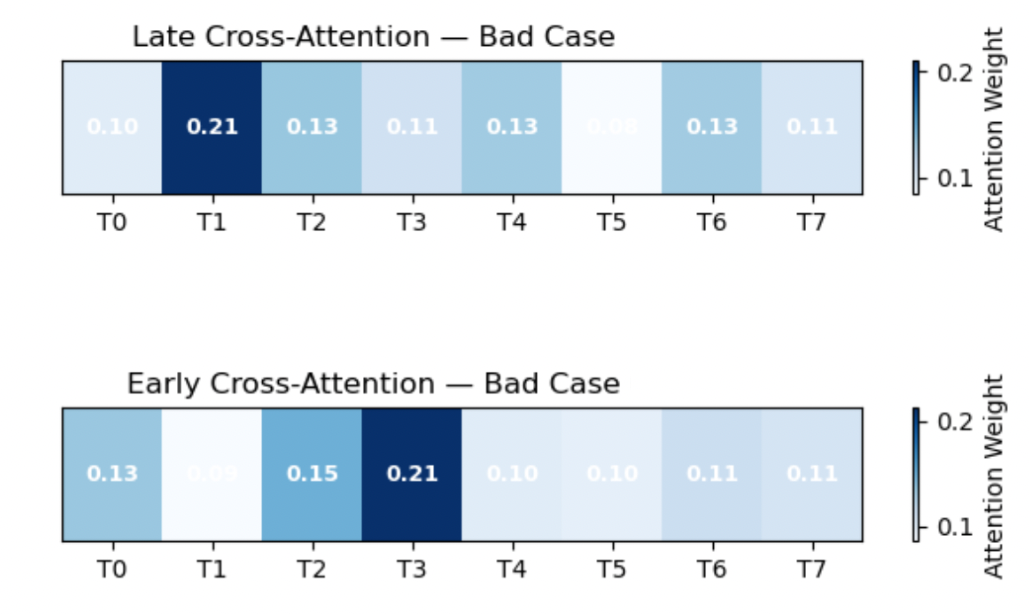
\includegraphics[width=0.8\textwidth]{Bilder/attention_bad_case.png}
    \caption{Attention-Weights im Bad Case.}
    \label{fig:attention_bad_case}
\end{figure}

\begin{figure}[h]
    \centering
    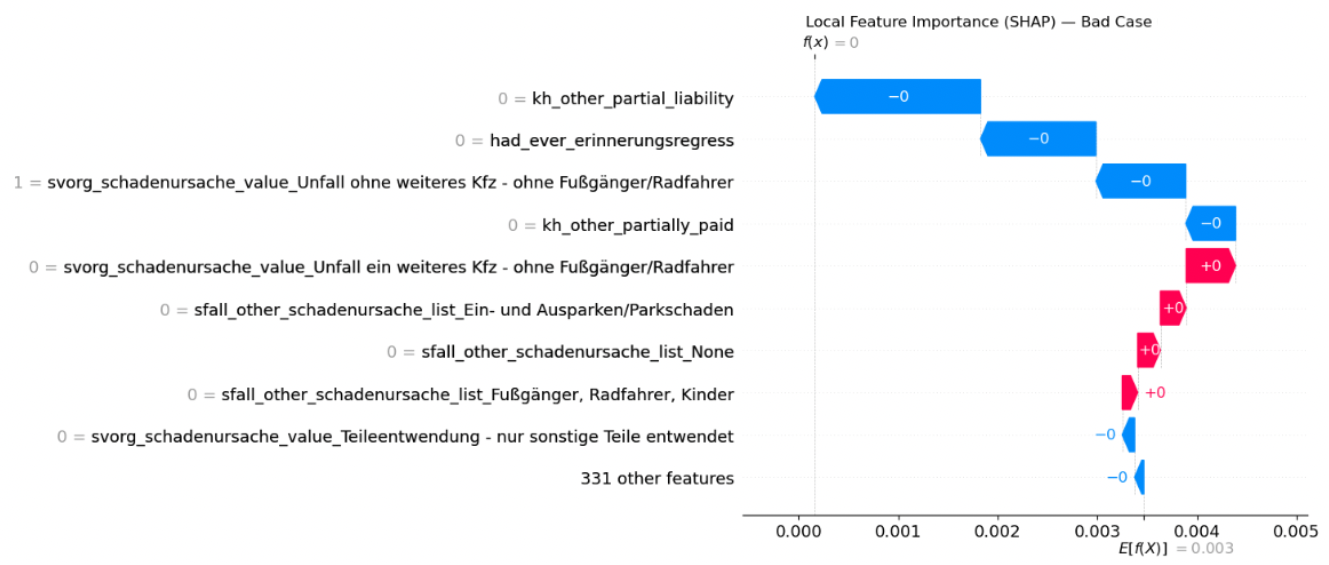
\includegraphics[width=0.8\textwidth]{Bilder/feature_importance_bad_case.png}
    \caption{Feature Importance (SHAP) im Bad Case.}
    \label{fig:feature_importance_bad_case}
\end{figure}
